% O16 plots

\label{DOMFits}

\section{Data used to constrain DOM fit of \oSix}
\label{O16DOMOutput}
\subsection{Positive-energy data}

\begin{figure}[H]
    \centering
    \begin{minipage}{0.45\textwidth}
        \centering
        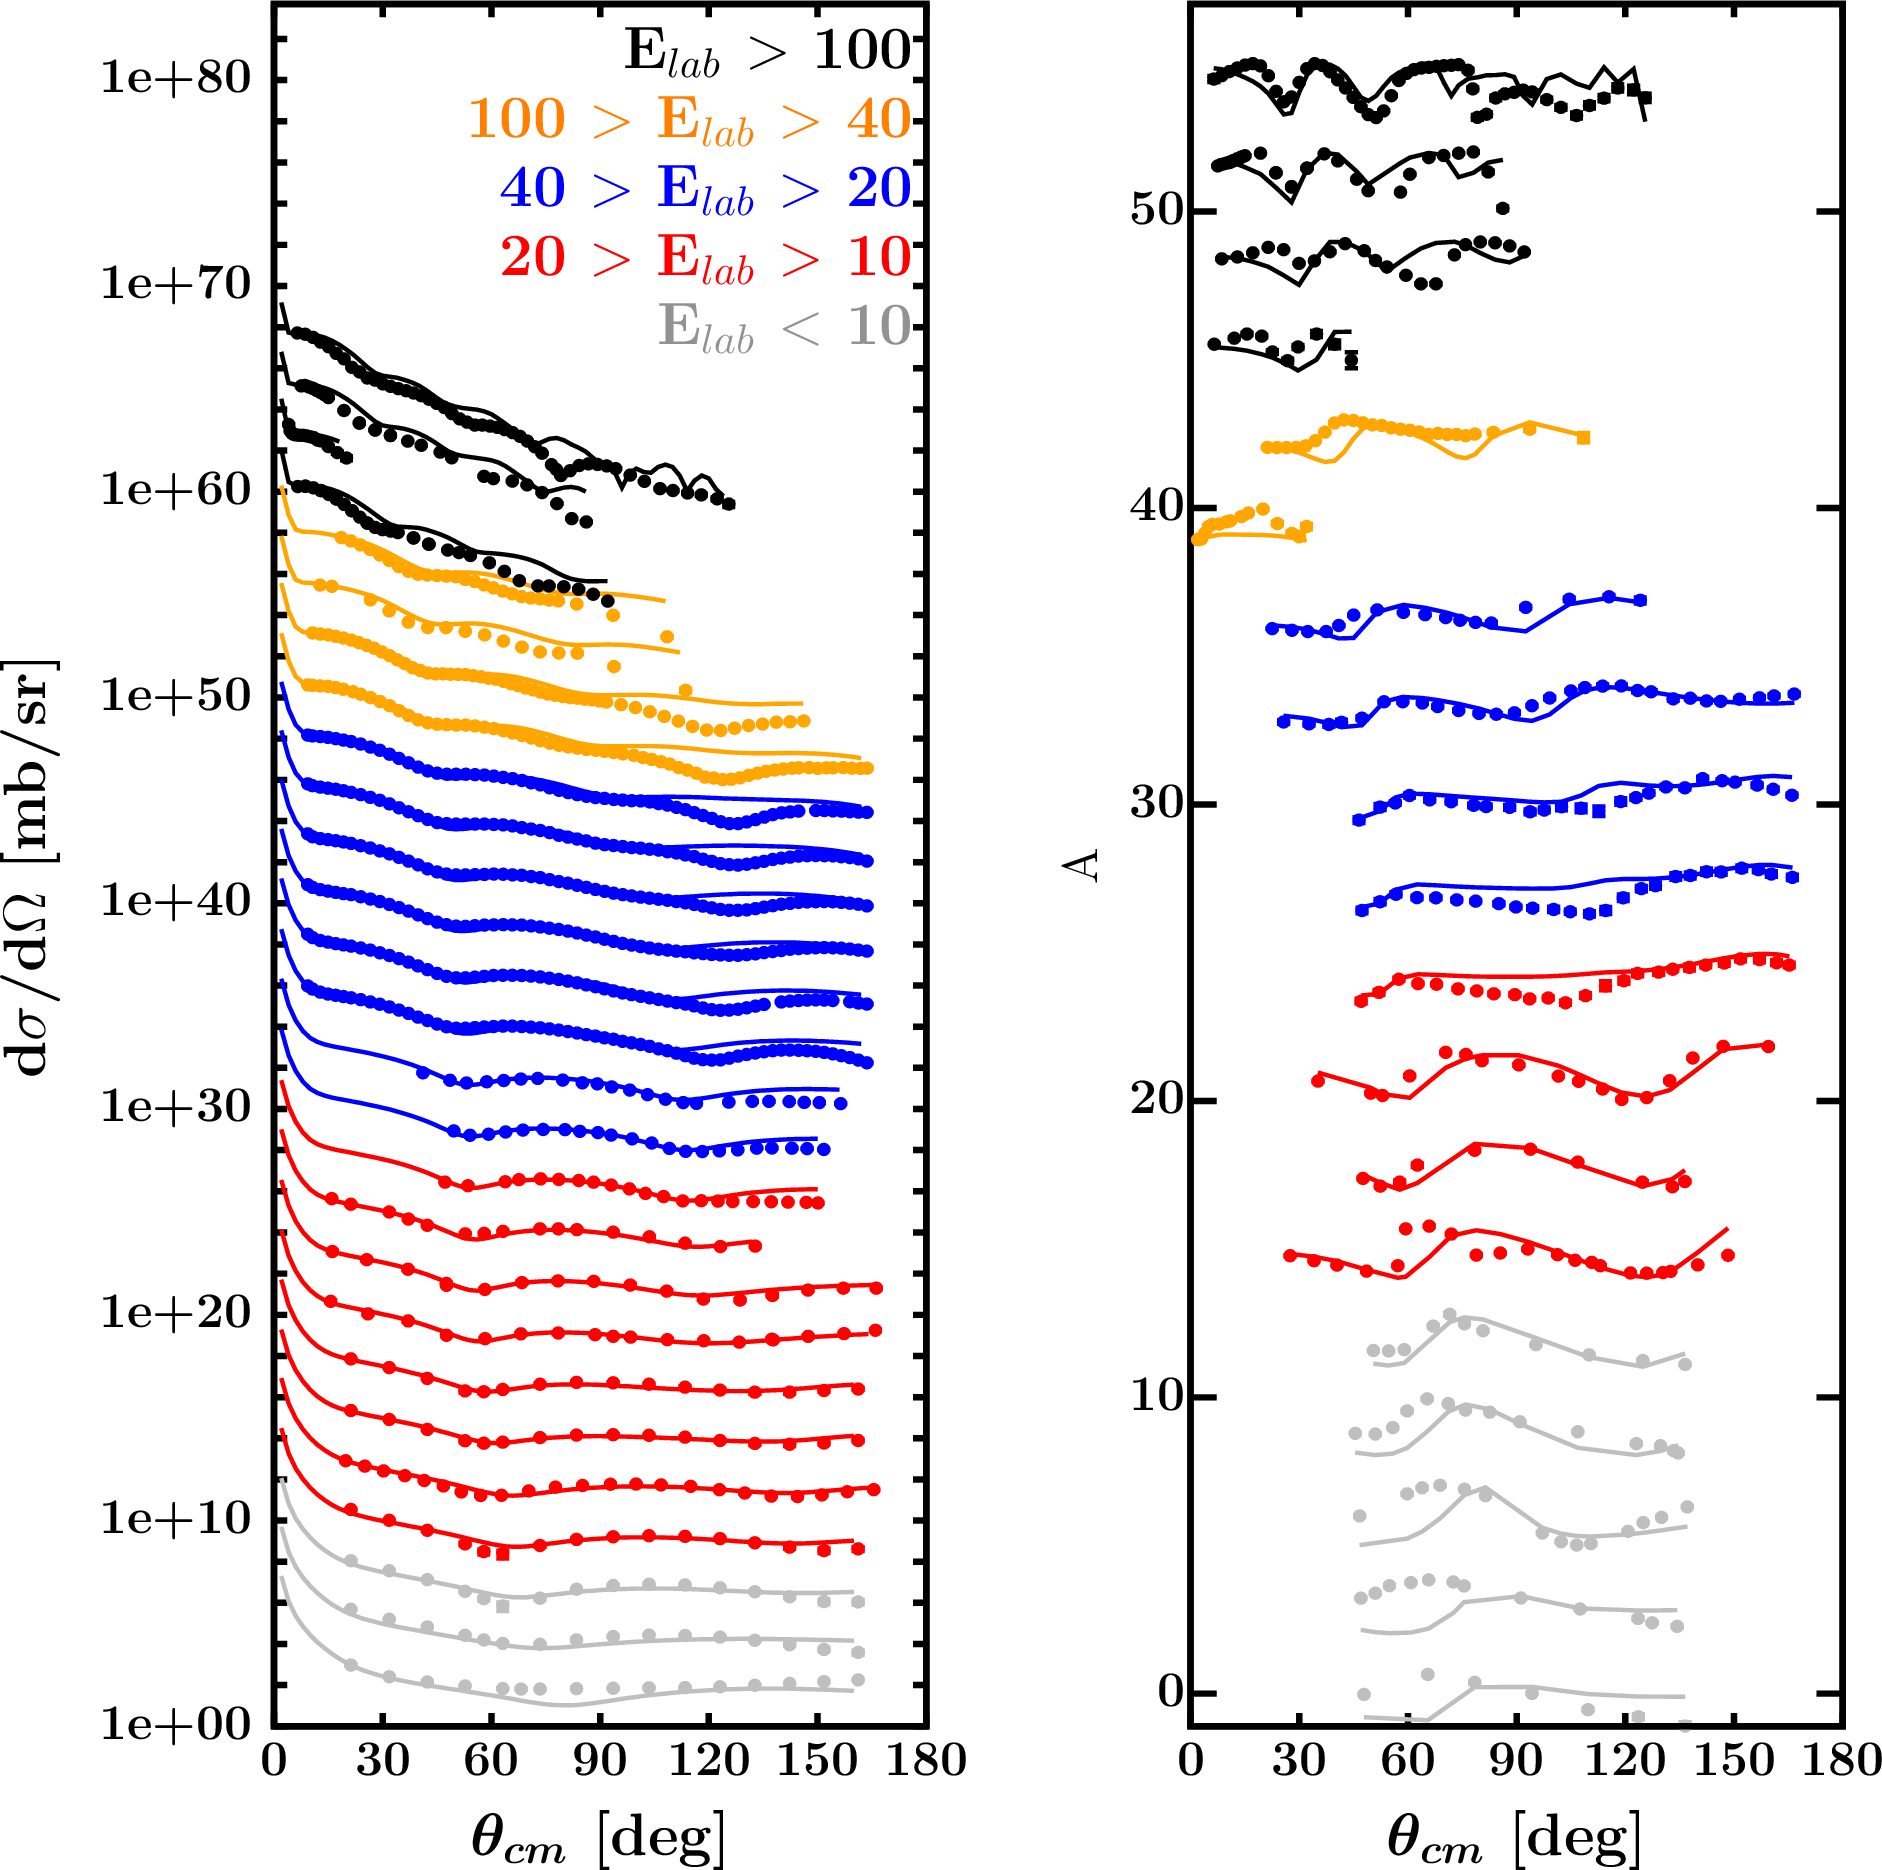
\includegraphics[width=1.0\textwidth]{figures/o16_protonElastic.png}
        \caption{Proton elastic scattering data}
        \label{DOMFitData_o16_proton_elastic}
    \end{minipage}\hfill
    \begin{minipage}{0.45\textwidth}
        \centering
        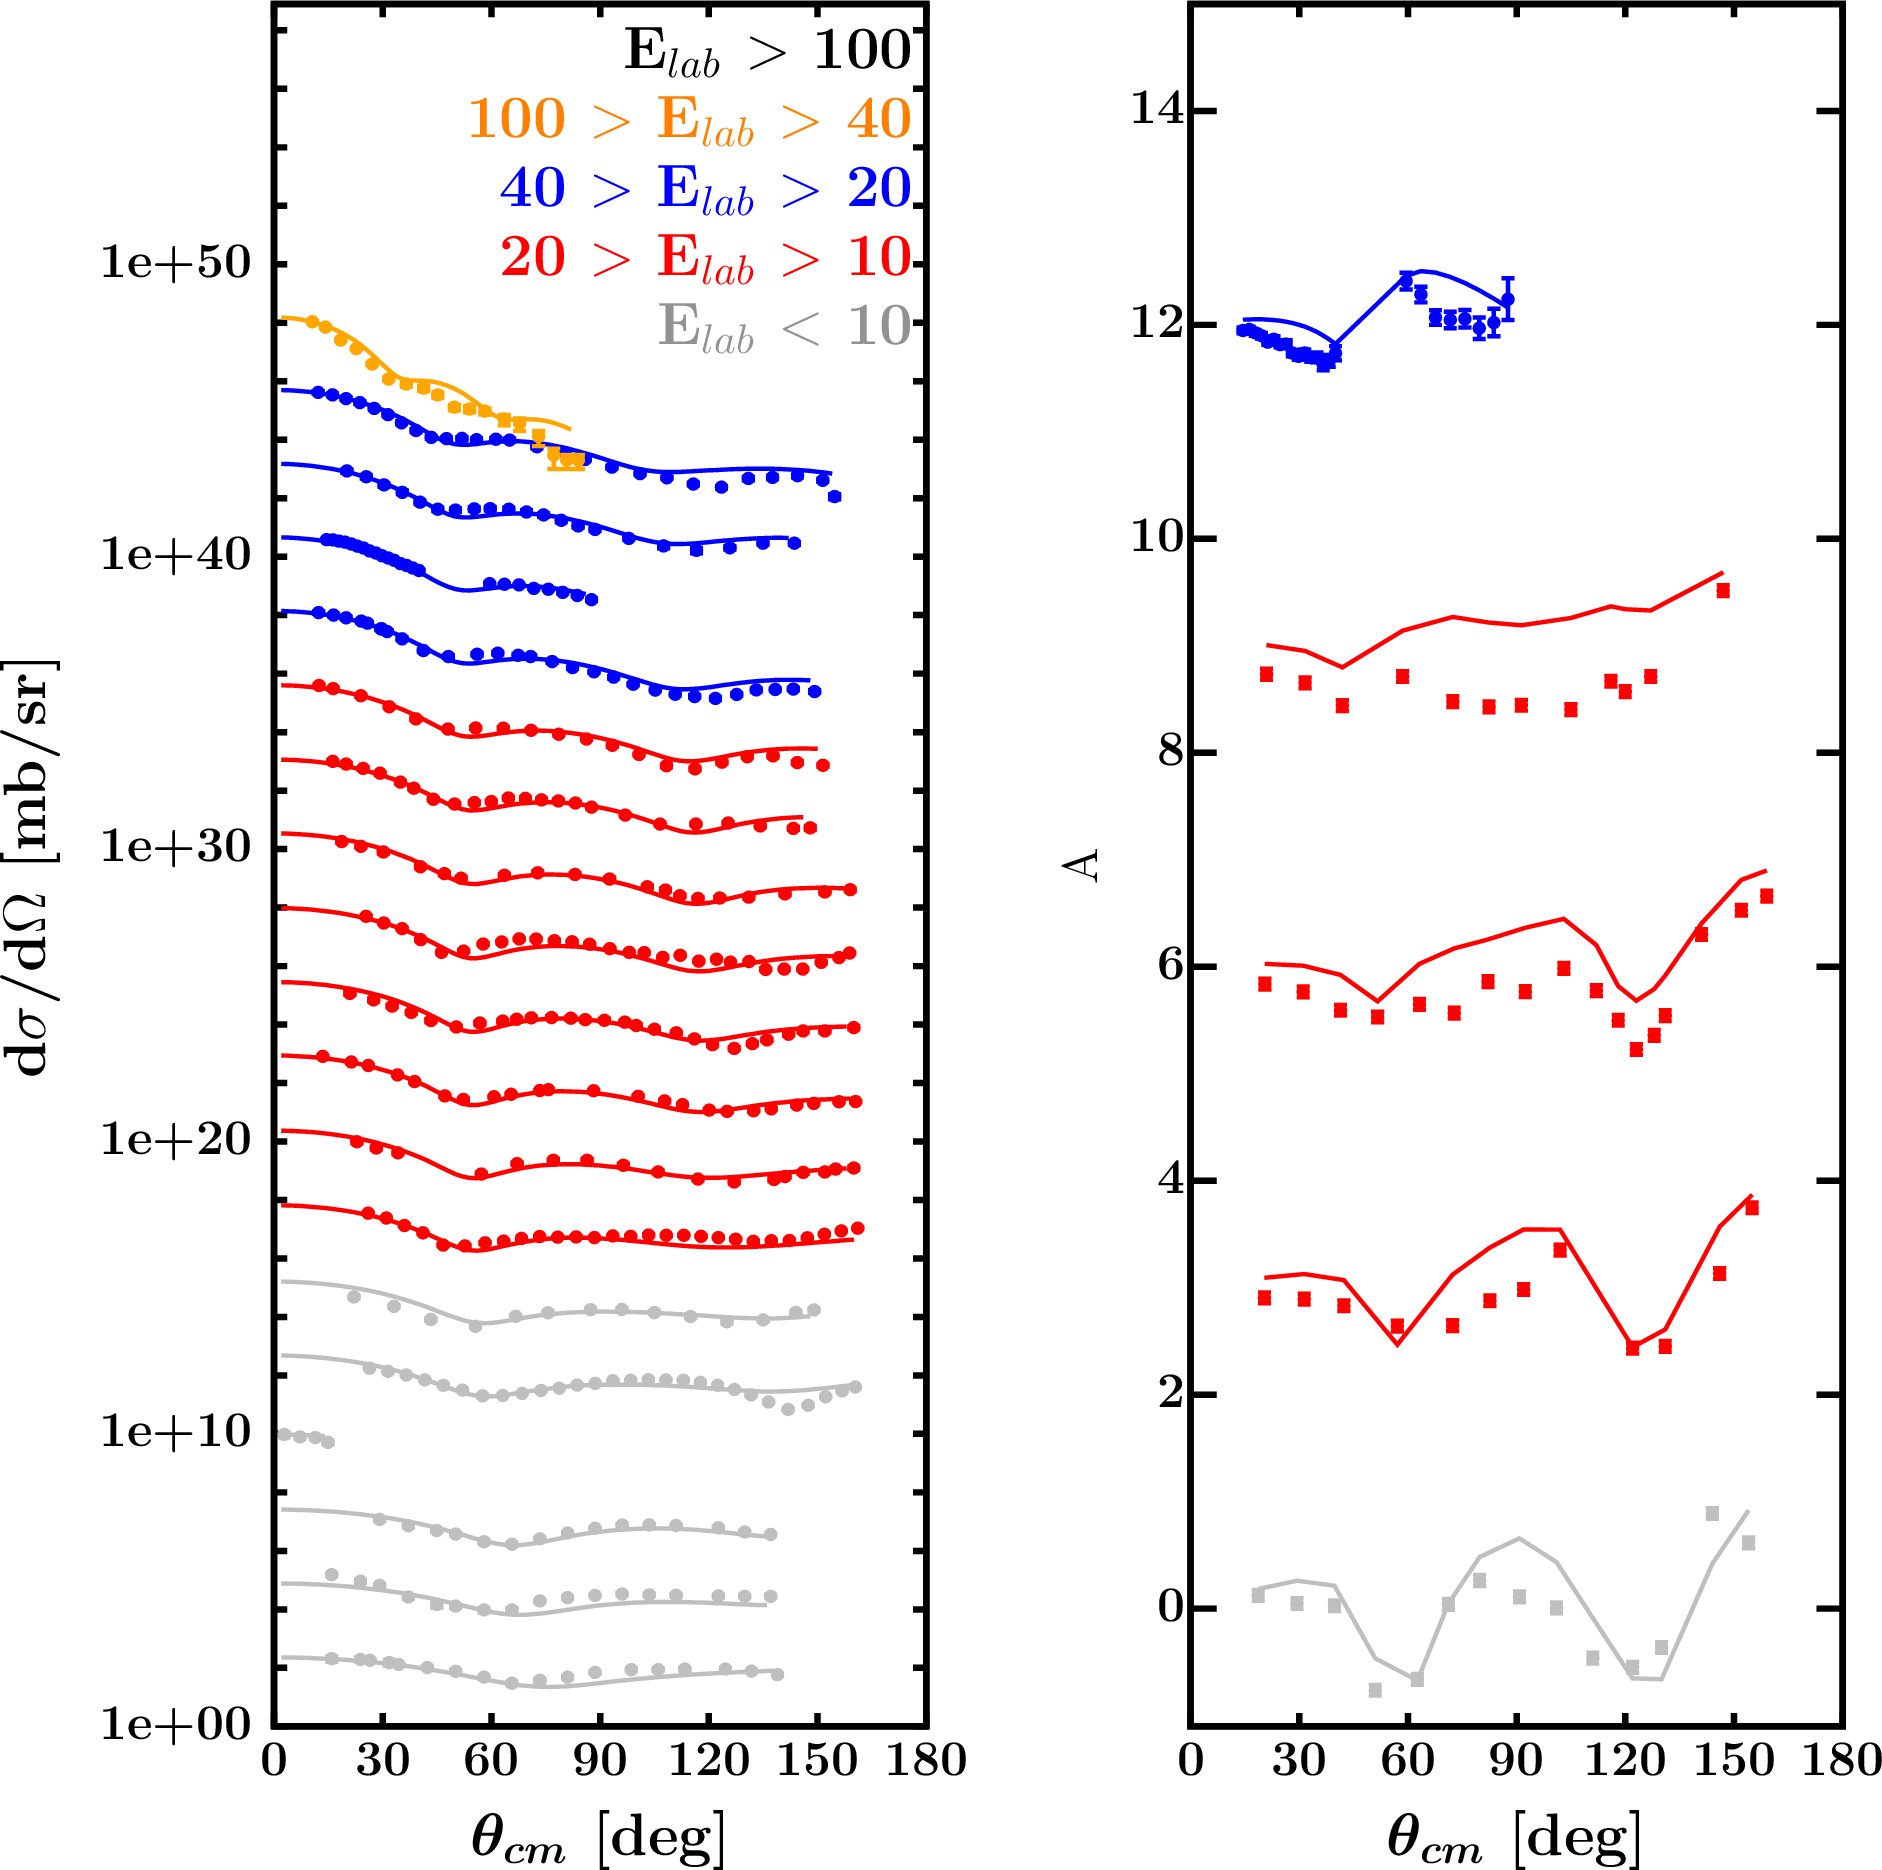
\includegraphics[width=1.0\textwidth]{figures/o16_neutronElastic.png}
        \caption{Neutron elastic scattering data}
        \label{DOMFitData_o16_neutron_elastic}
    \end{minipage}
\end{figure}

\begin{figure}[H]
    \centering
    \begin{minipage}{0.45\textwidth}
        \centering
        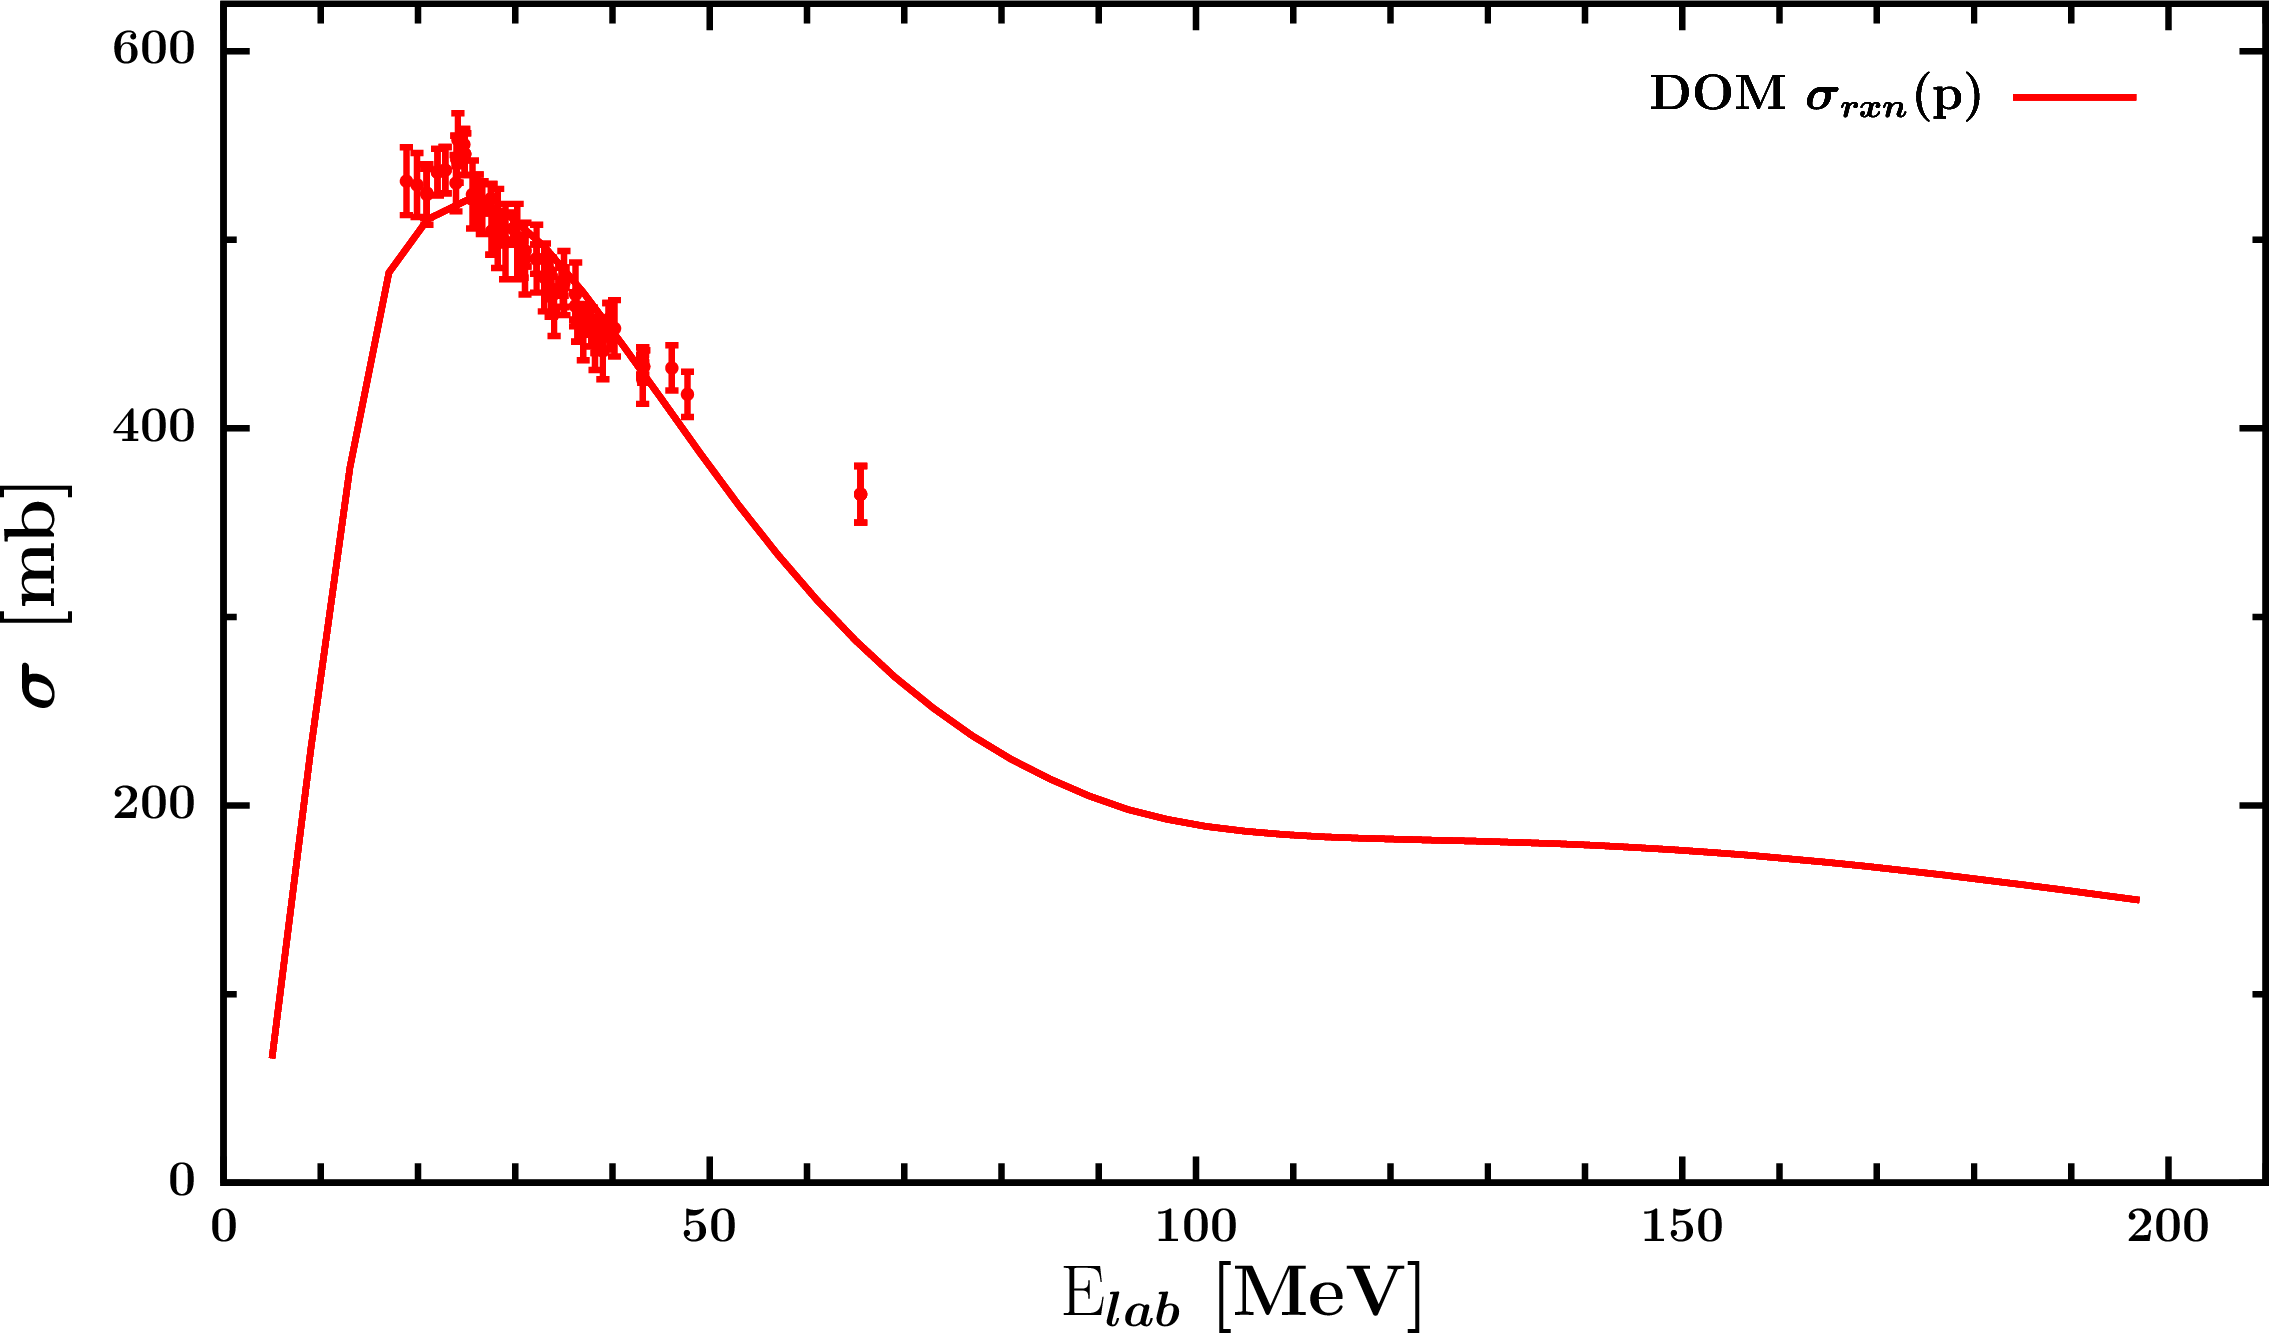
\includegraphics[width=1.0\textwidth]{figures/o16_protonInelastic.png}
        \caption{Proton \rxn data}
        \label{DOMFitData_o16_proton_inelastic}
    \end{minipage}\hfill
    \begin{minipage}{0.45\textwidth}
        \centering
        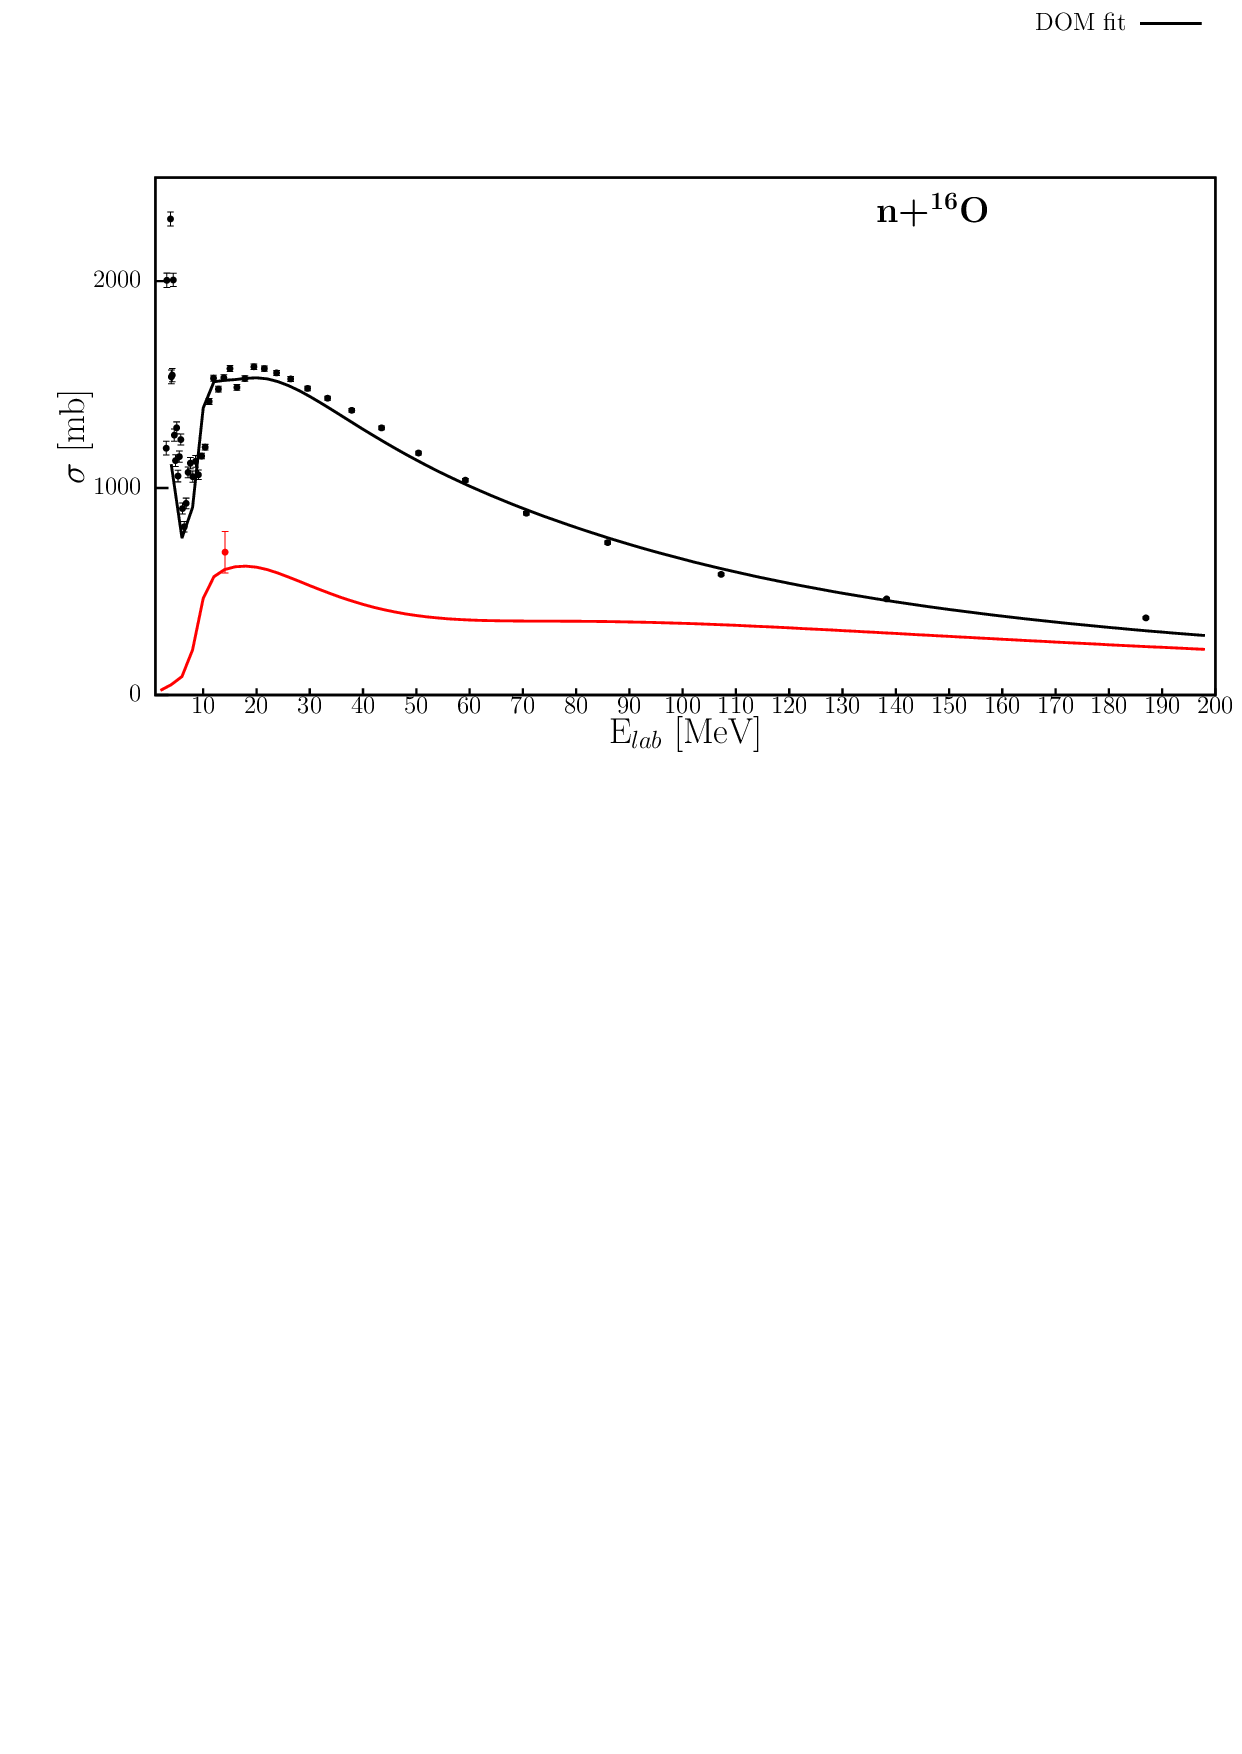
\includegraphics[width=1.0\textwidth]{figures/o16_neutronInelastic.png}
        \caption{Neutron \rxn and \tot data}
        \label{DOMFitData_o16_neutron_inelastic}
    \end{minipage}
\end{figure}

\afterpage{\clearpage}

\subsection{Negative-energy data}

\begin{figure}[H]
    \centering
    \begin{minipage}{0.45\textwidth}
        \centering
        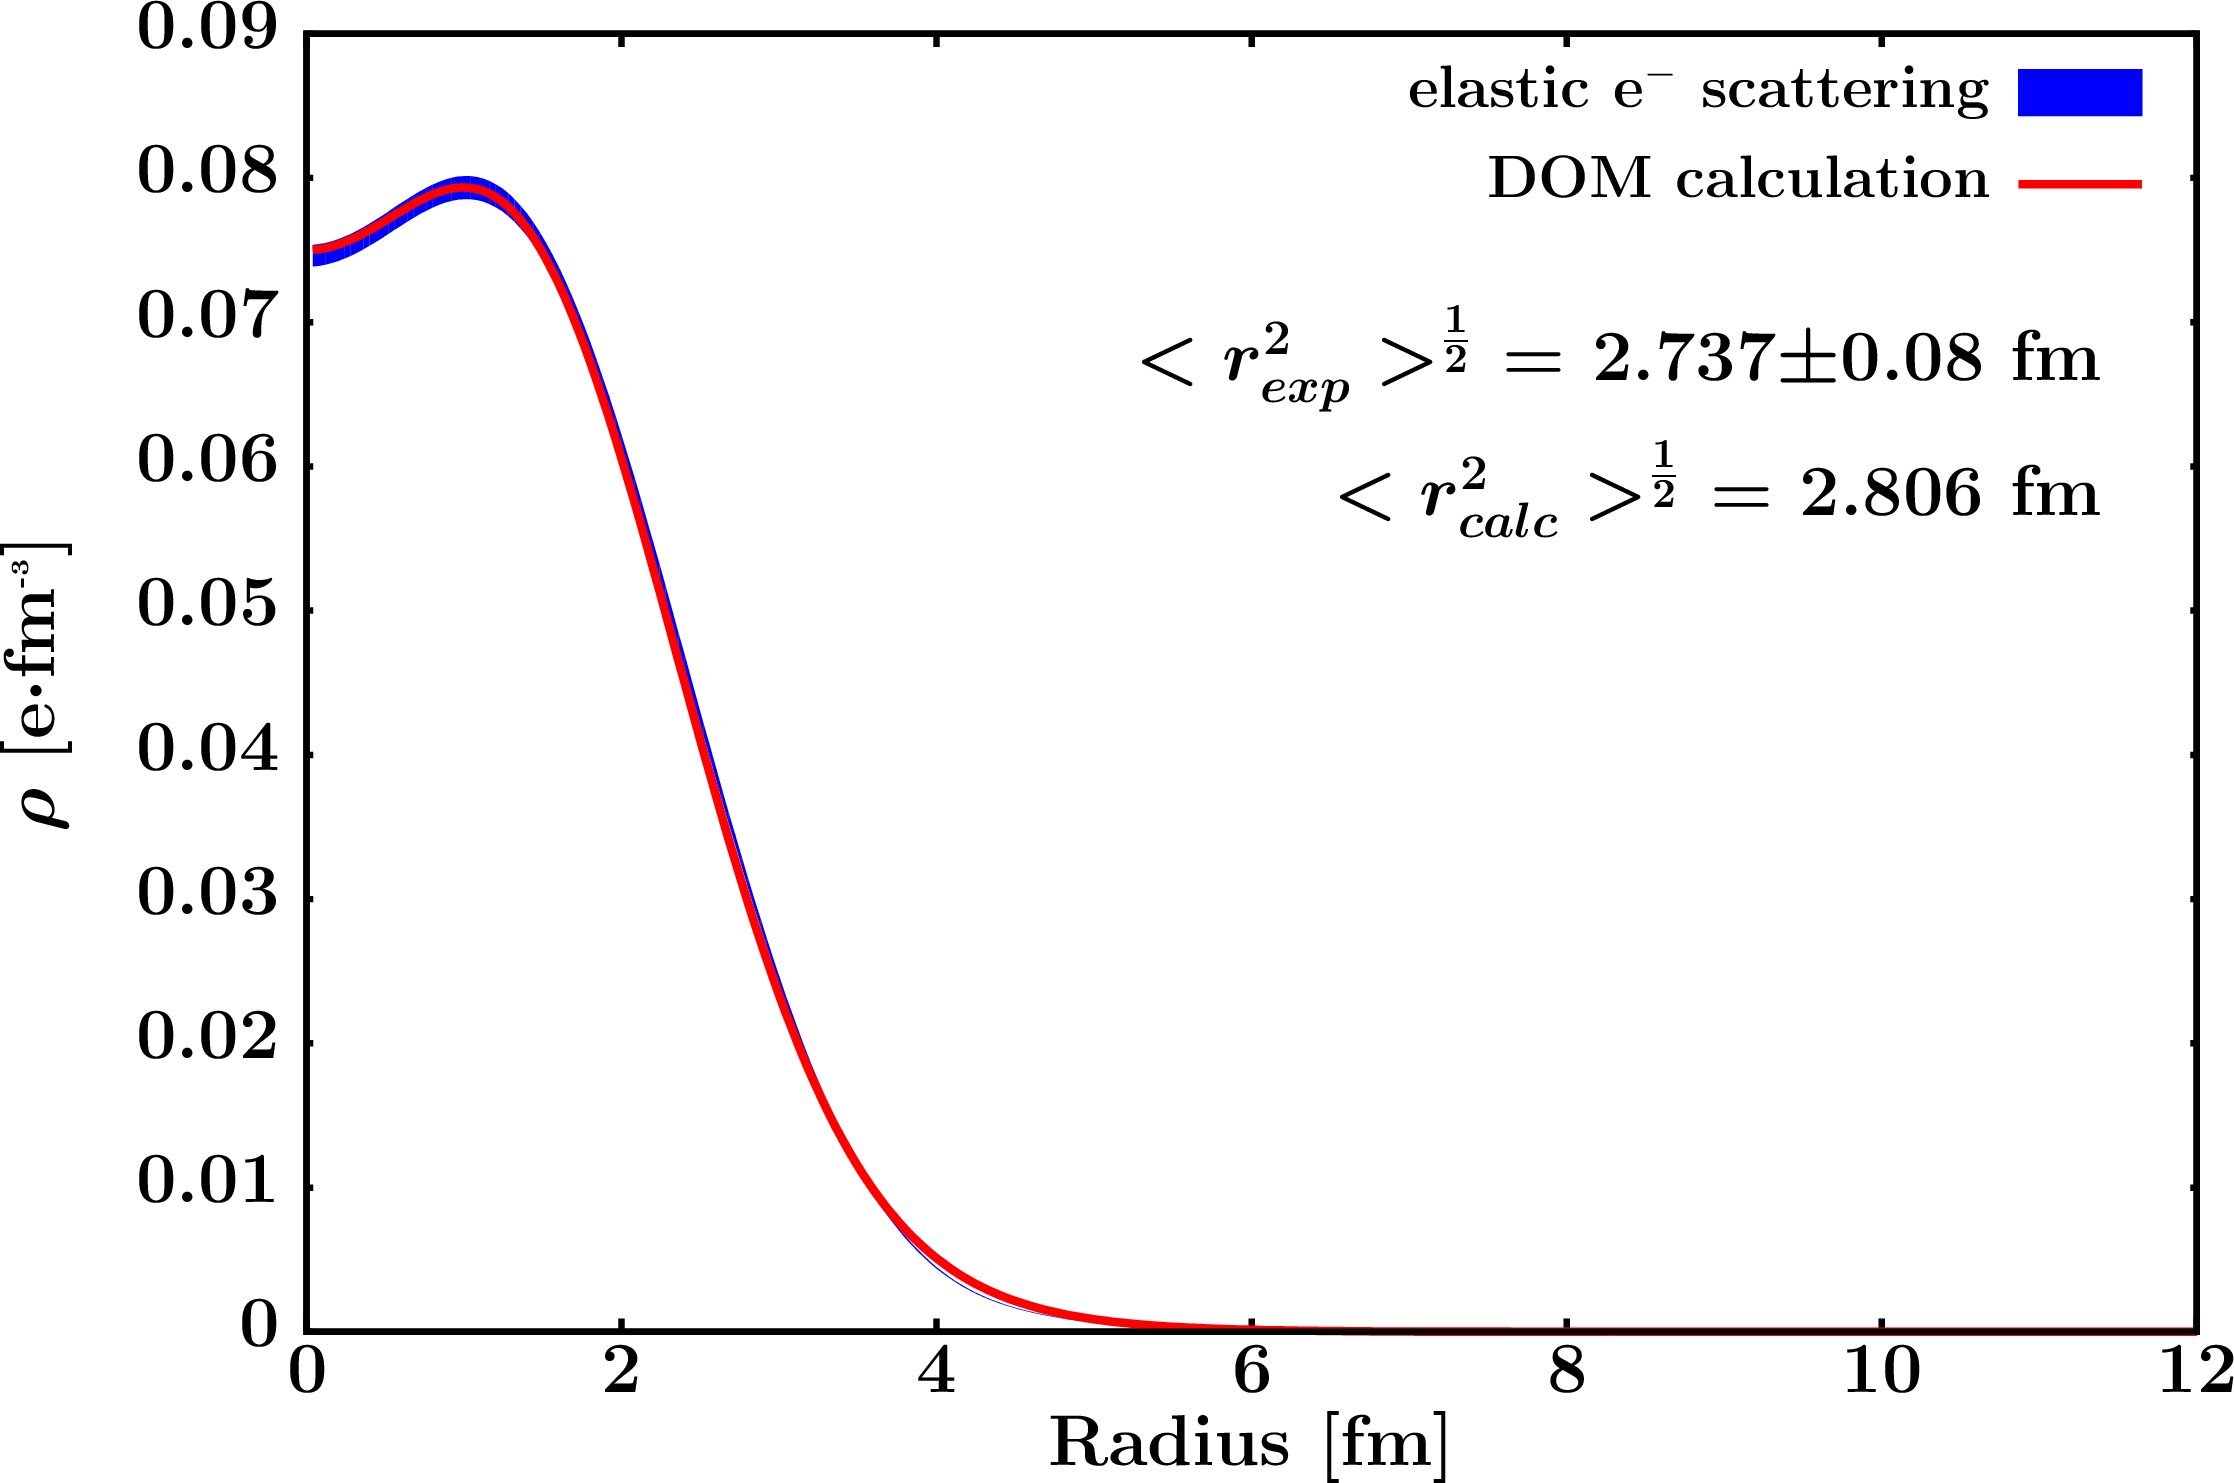
\includegraphics[width=1.0\textwidth]{figures/o16_chargeDensity.png}
        \caption{Charge density data}
        \label{DOMFitData_o16_chargeDensity}
    \end{minipage}\hfill
    \begin{minipage}{0.45\textwidth}
        \centering
        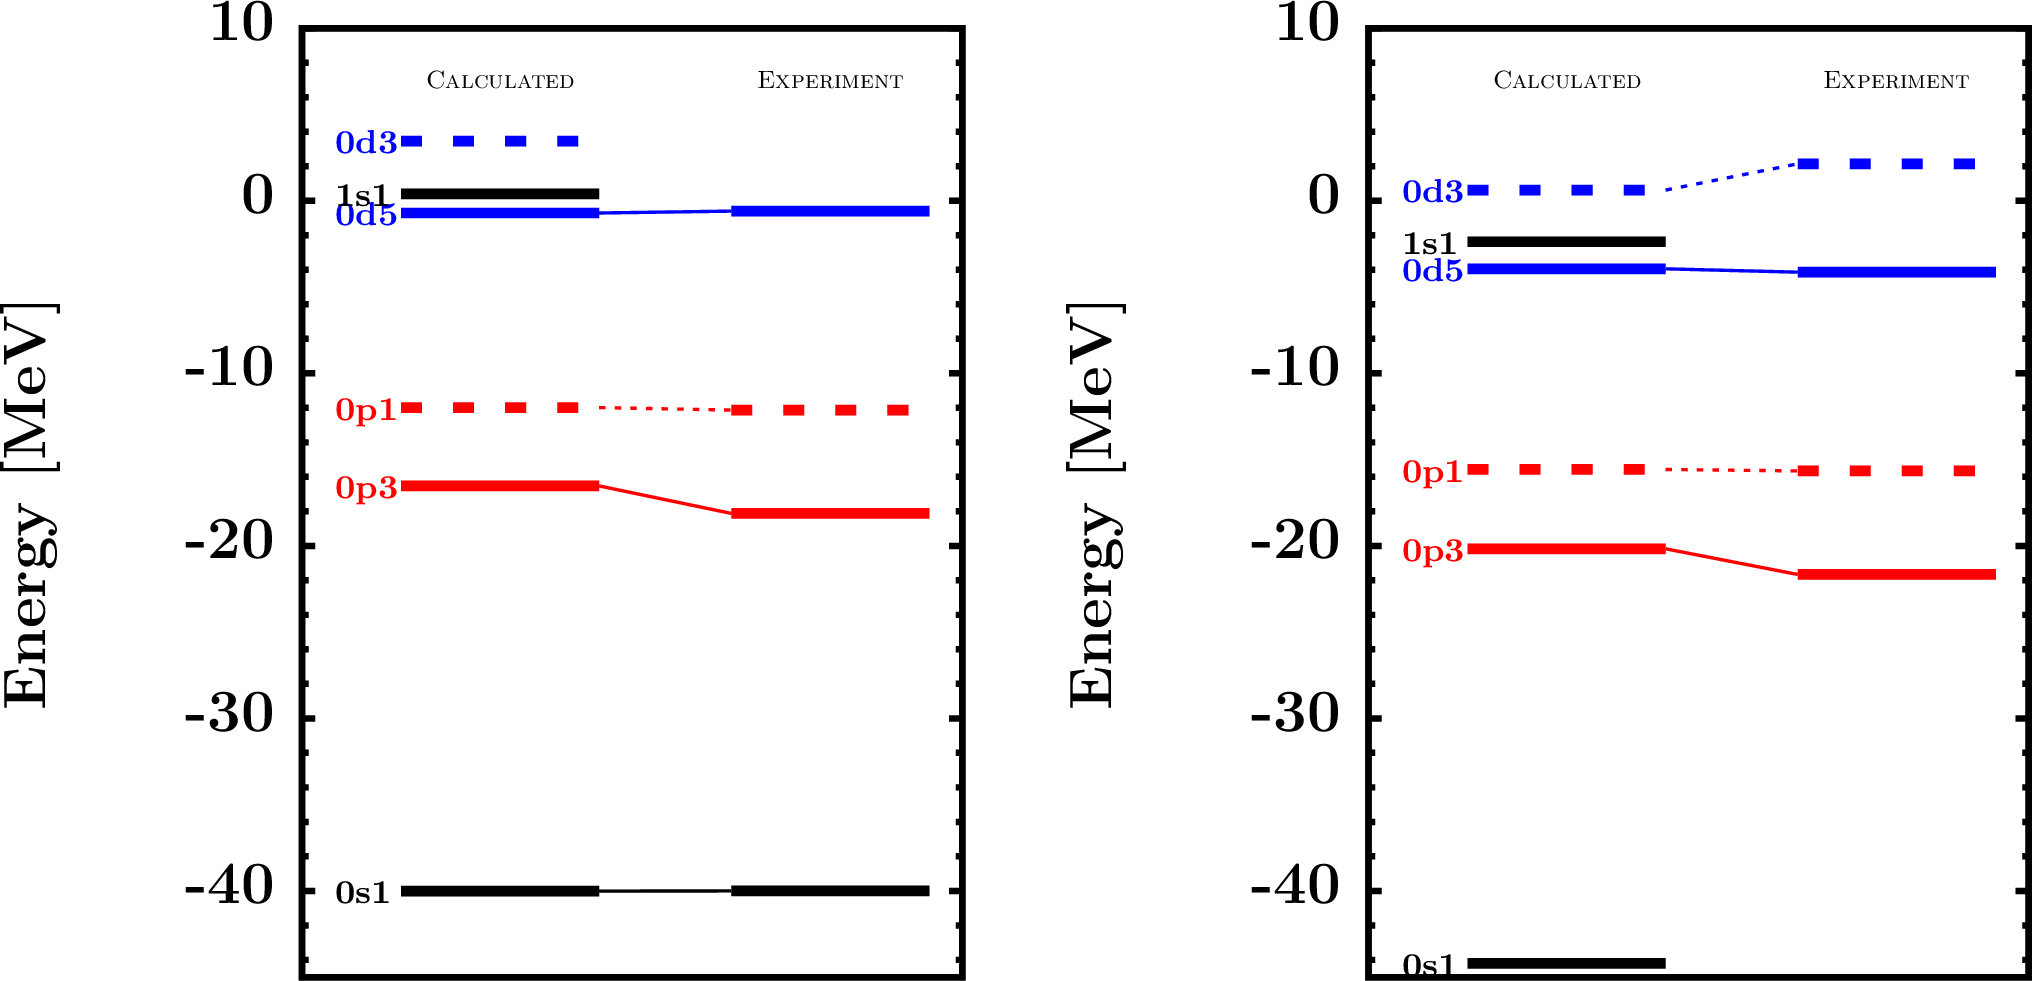
\includegraphics[width=1.0\textwidth]{figures/o16_SPLevels.png}
        \caption{Single-particle levels}
        \label{DOMFitData_o16_SPLevels}
    \end{minipage}
\end{figure}

\afterpage{\clearpage}

\subsection{Visualization of extracted potential}

\begin{figure}[H]
    \centering
    \begin{minipage}{0.45\textwidth}
        \centering
        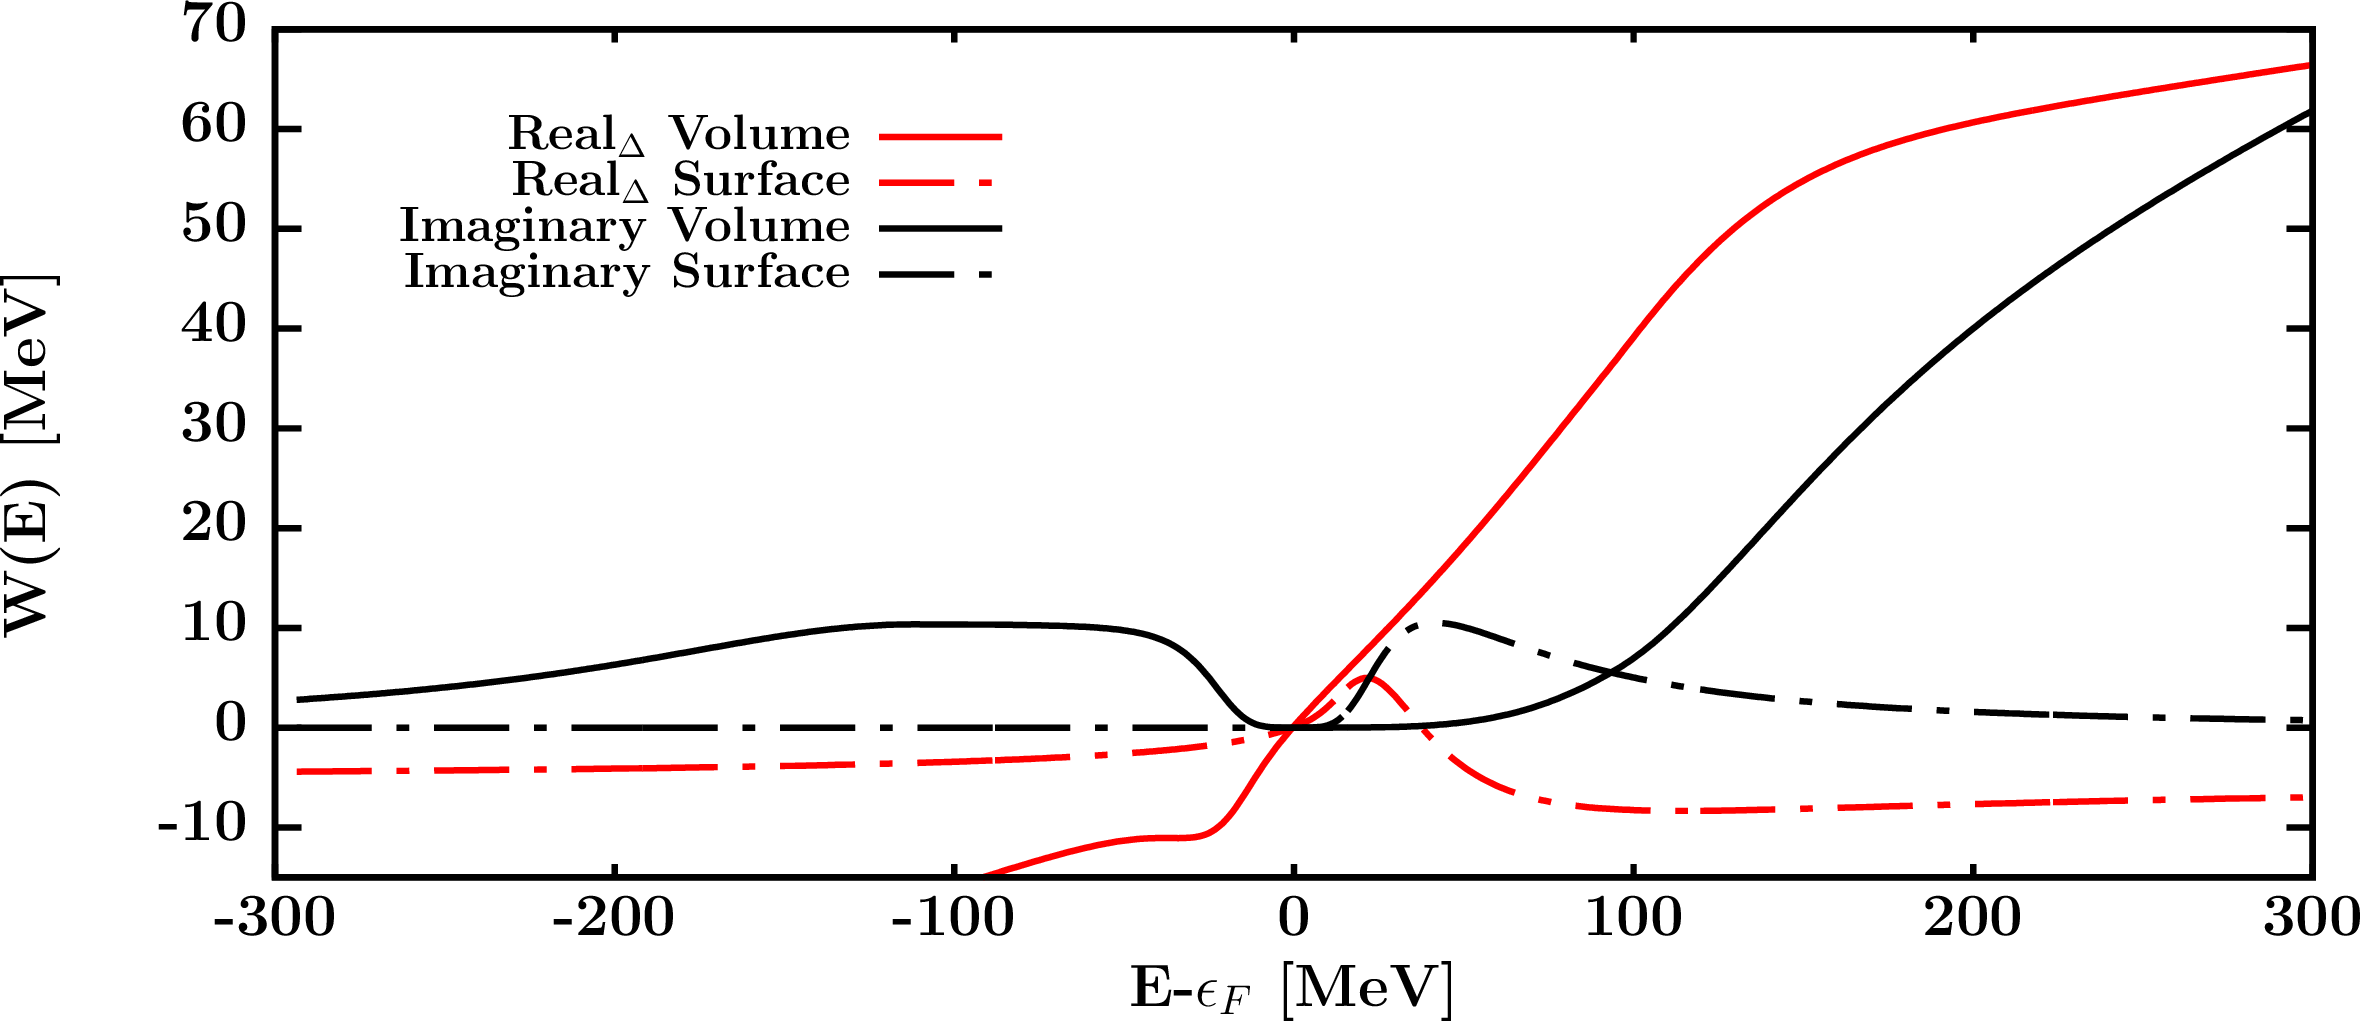
\includegraphics[width=1.0\textwidth]{figures/o16_protonPotentials.png}
        \caption{Energy-dependence of optical potential components for protons
        on \oSix}
        \label{DOMFitData_o16_proton_potentialComponent_energy}
    \end{minipage}\hfill
    \begin{minipage}{0.45\textwidth}
        \centering
        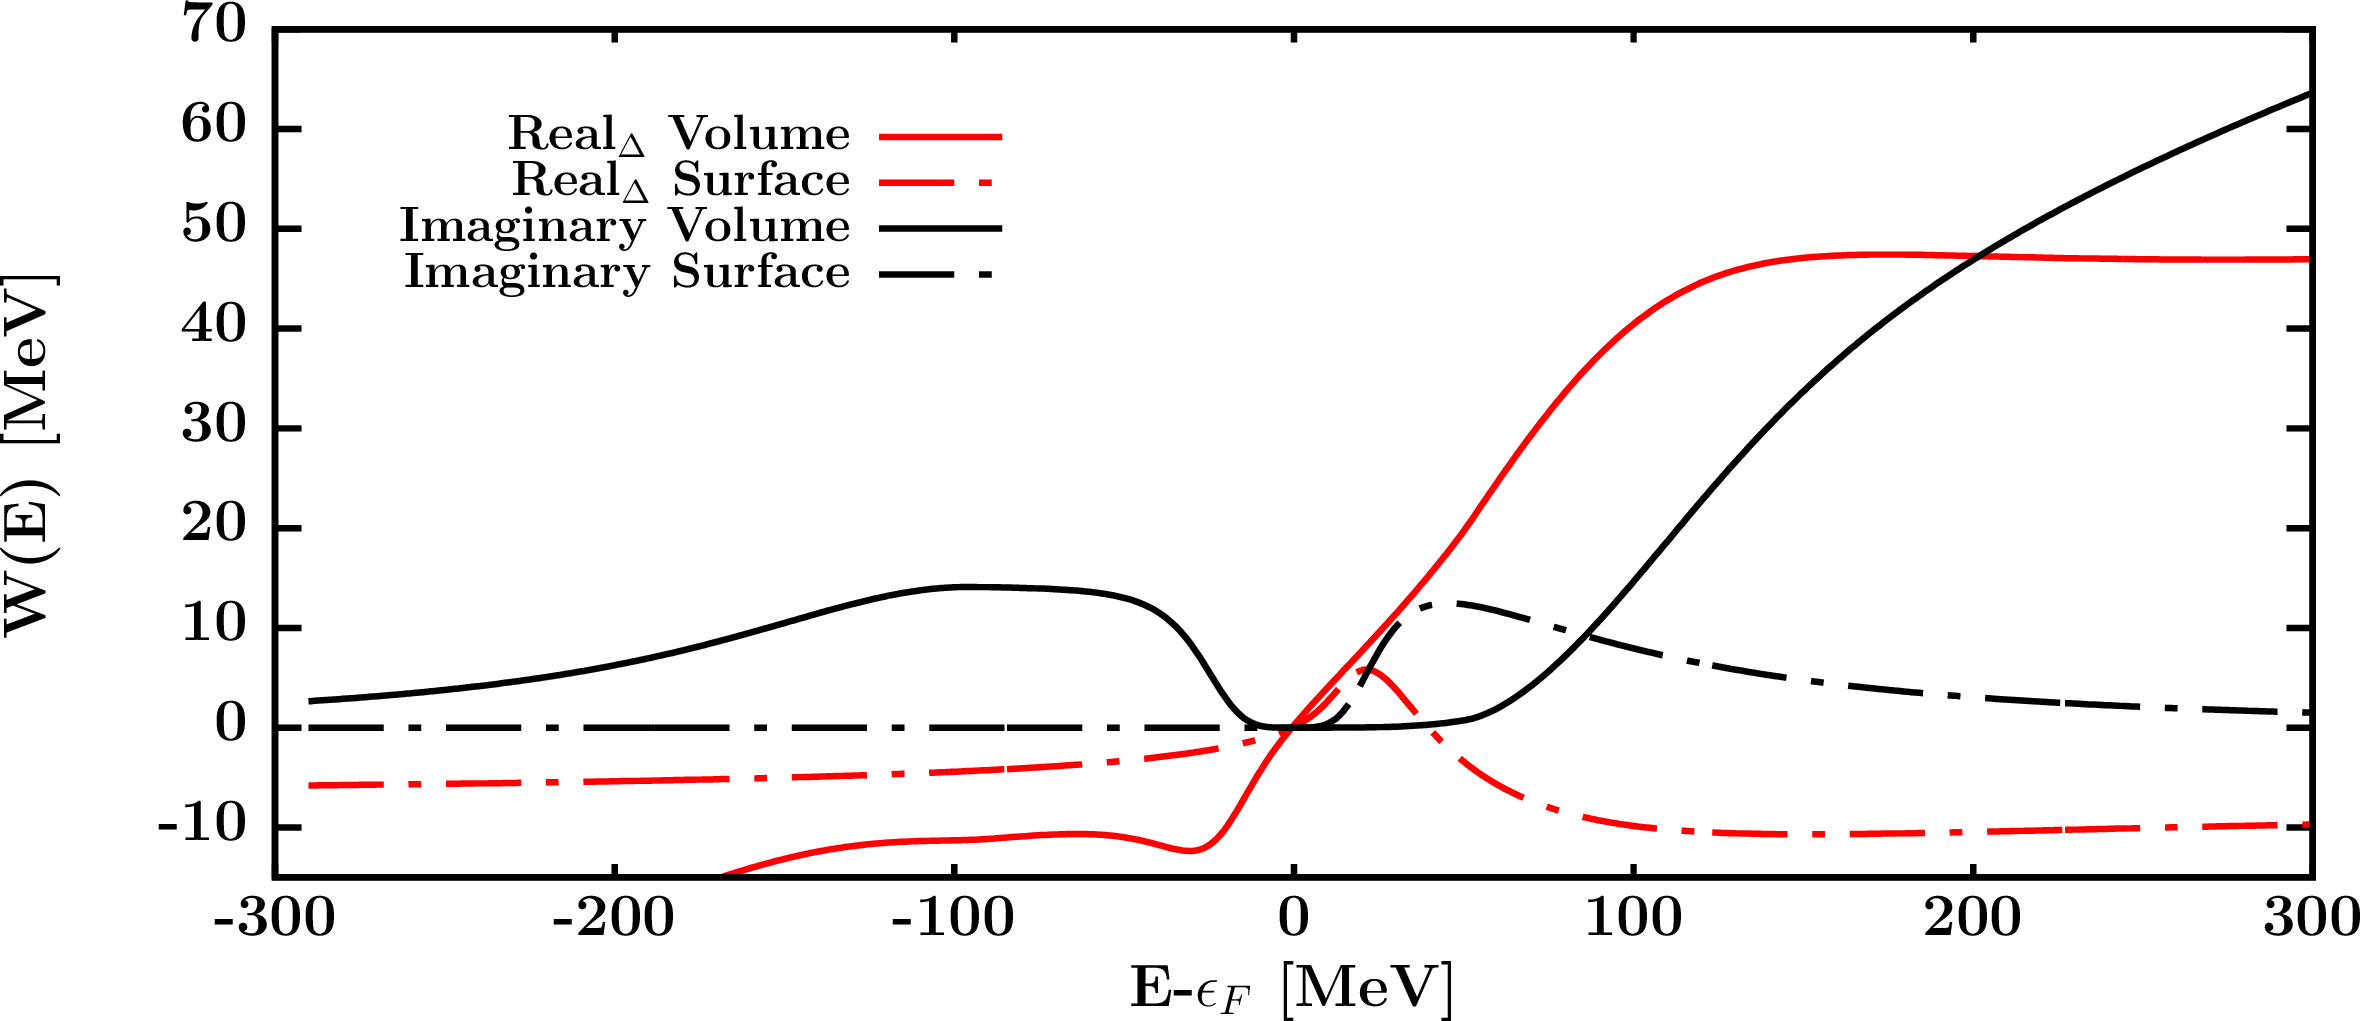
\includegraphics[width=1.0\textwidth]{figures/o16_neutronPotentials.png}
        \caption{Neutron potential energy-dependent component}
        \label{DOMFitData_o16_neutron_potentialComponent_energy}
    \end{minipage}
\end{figure}

\begin{figure}[H]
    \centering
    \begin{minipage}{0.45\textwidth}
        \centering
        
\includegraphics[width=1.0\textwidth]{figures/o16_protonVolumeIntegrals.png}
        \caption{Proton potential, integrated over r-space}
        \label{DOMFitData_o16_proton_potentialIntegral}
    \end{minipage}\hfill
    \begin{minipage}{0.45\textwidth}
        \centering
        
\includegraphics[width=1.0\textwidth]{figures/o16_neutronVolumeIntegrals.png}
        \caption{Neutron potential, integrated over r-space}
        \label{DOMFitData_o16_neutron_potentialIntegral}
    \end{minipage}
\end{figure}

\afterpage{\clearpage}

\subsection{Quantities of interest extracted from potential}

\begin{figure}[H]
    \centering
    \begin{minipage}{0.45\textwidth}
        \centering
        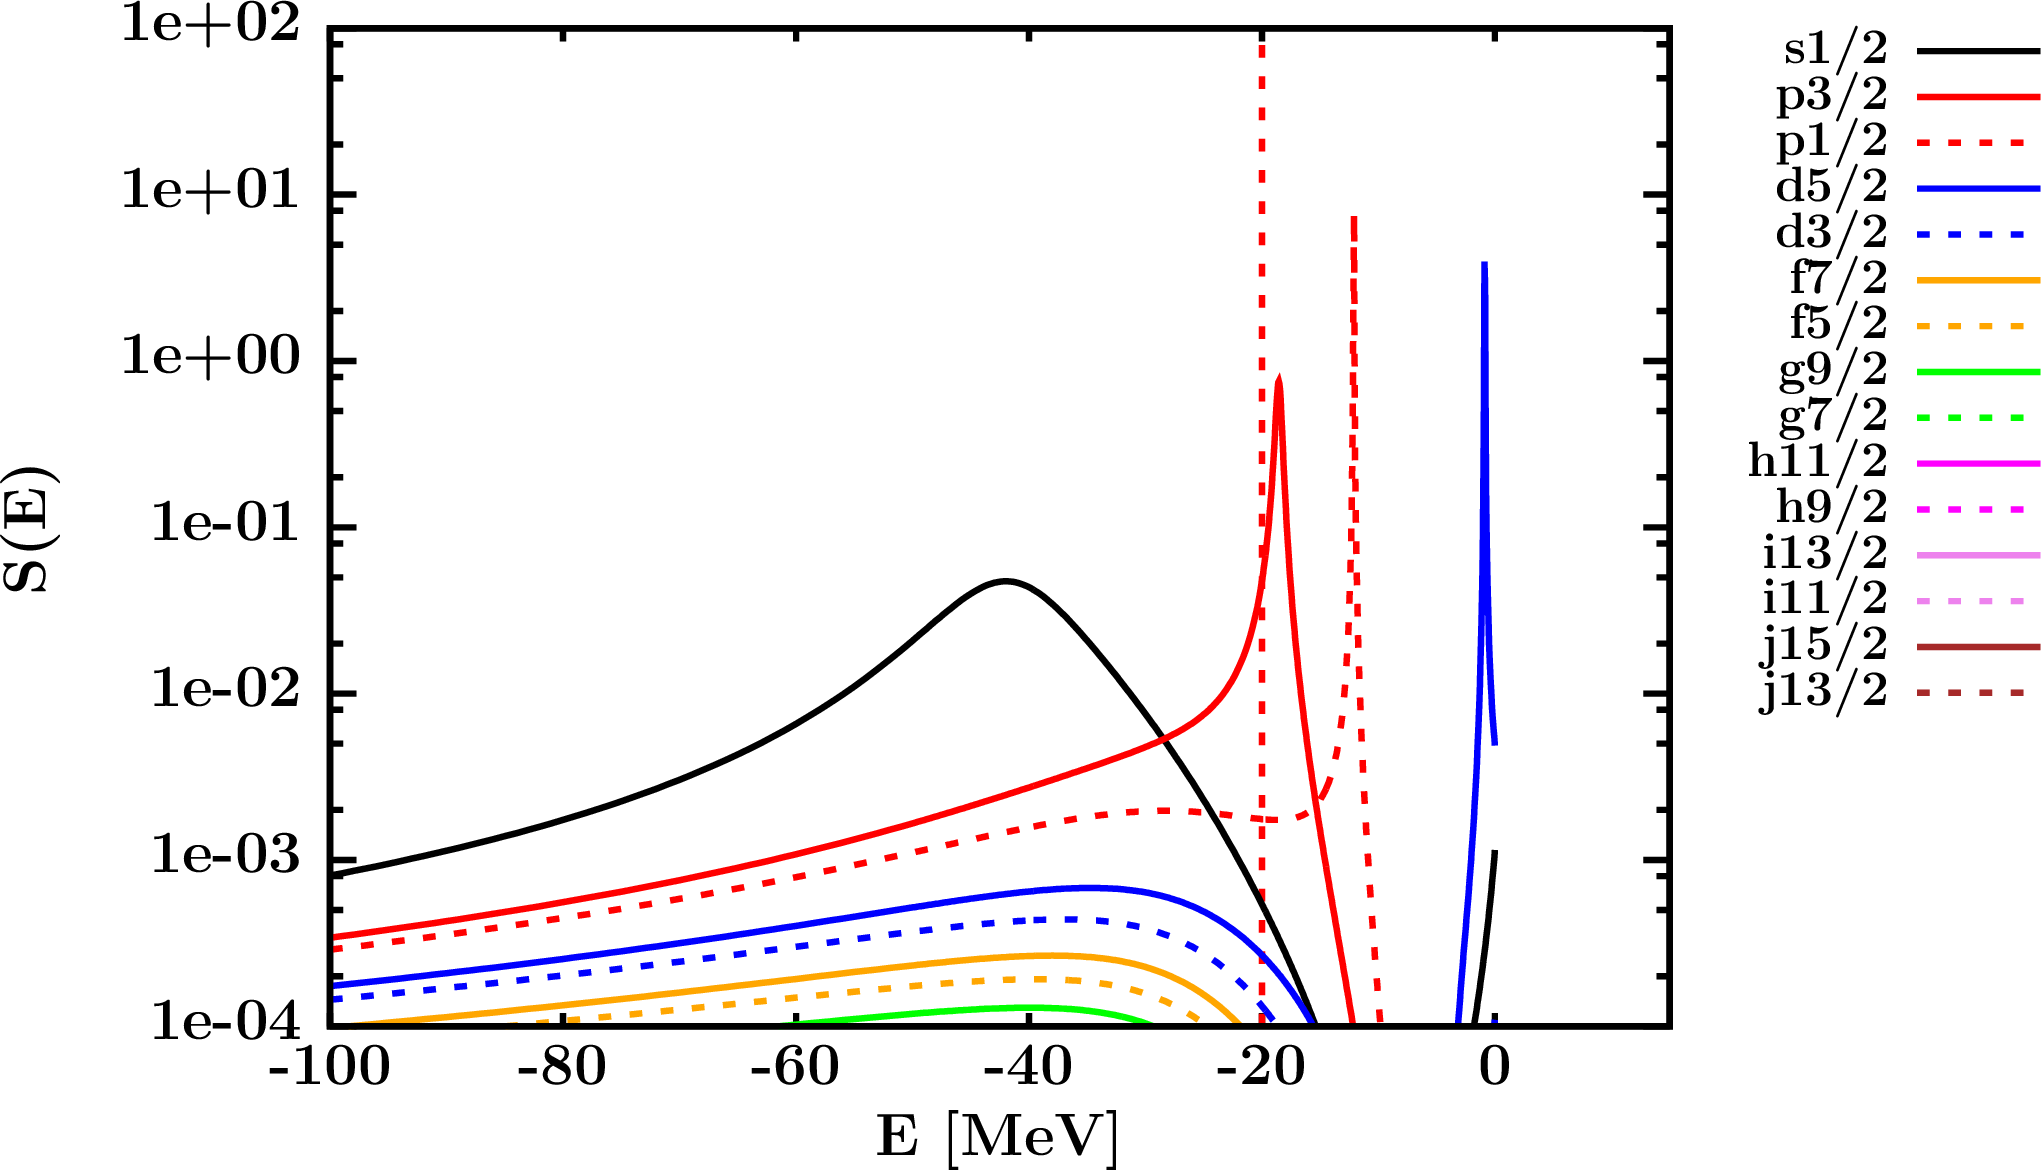
\includegraphics[width=1.0\textwidth]{figures/o16_protonSpectralFunctions.png}
        \caption{Proton spectral functions}
        \label{DOMFitData_o16_proton_spectralFunctions}
    \end{minipage}\hfill
    \begin{minipage}{0.45\textwidth}
        \centering
        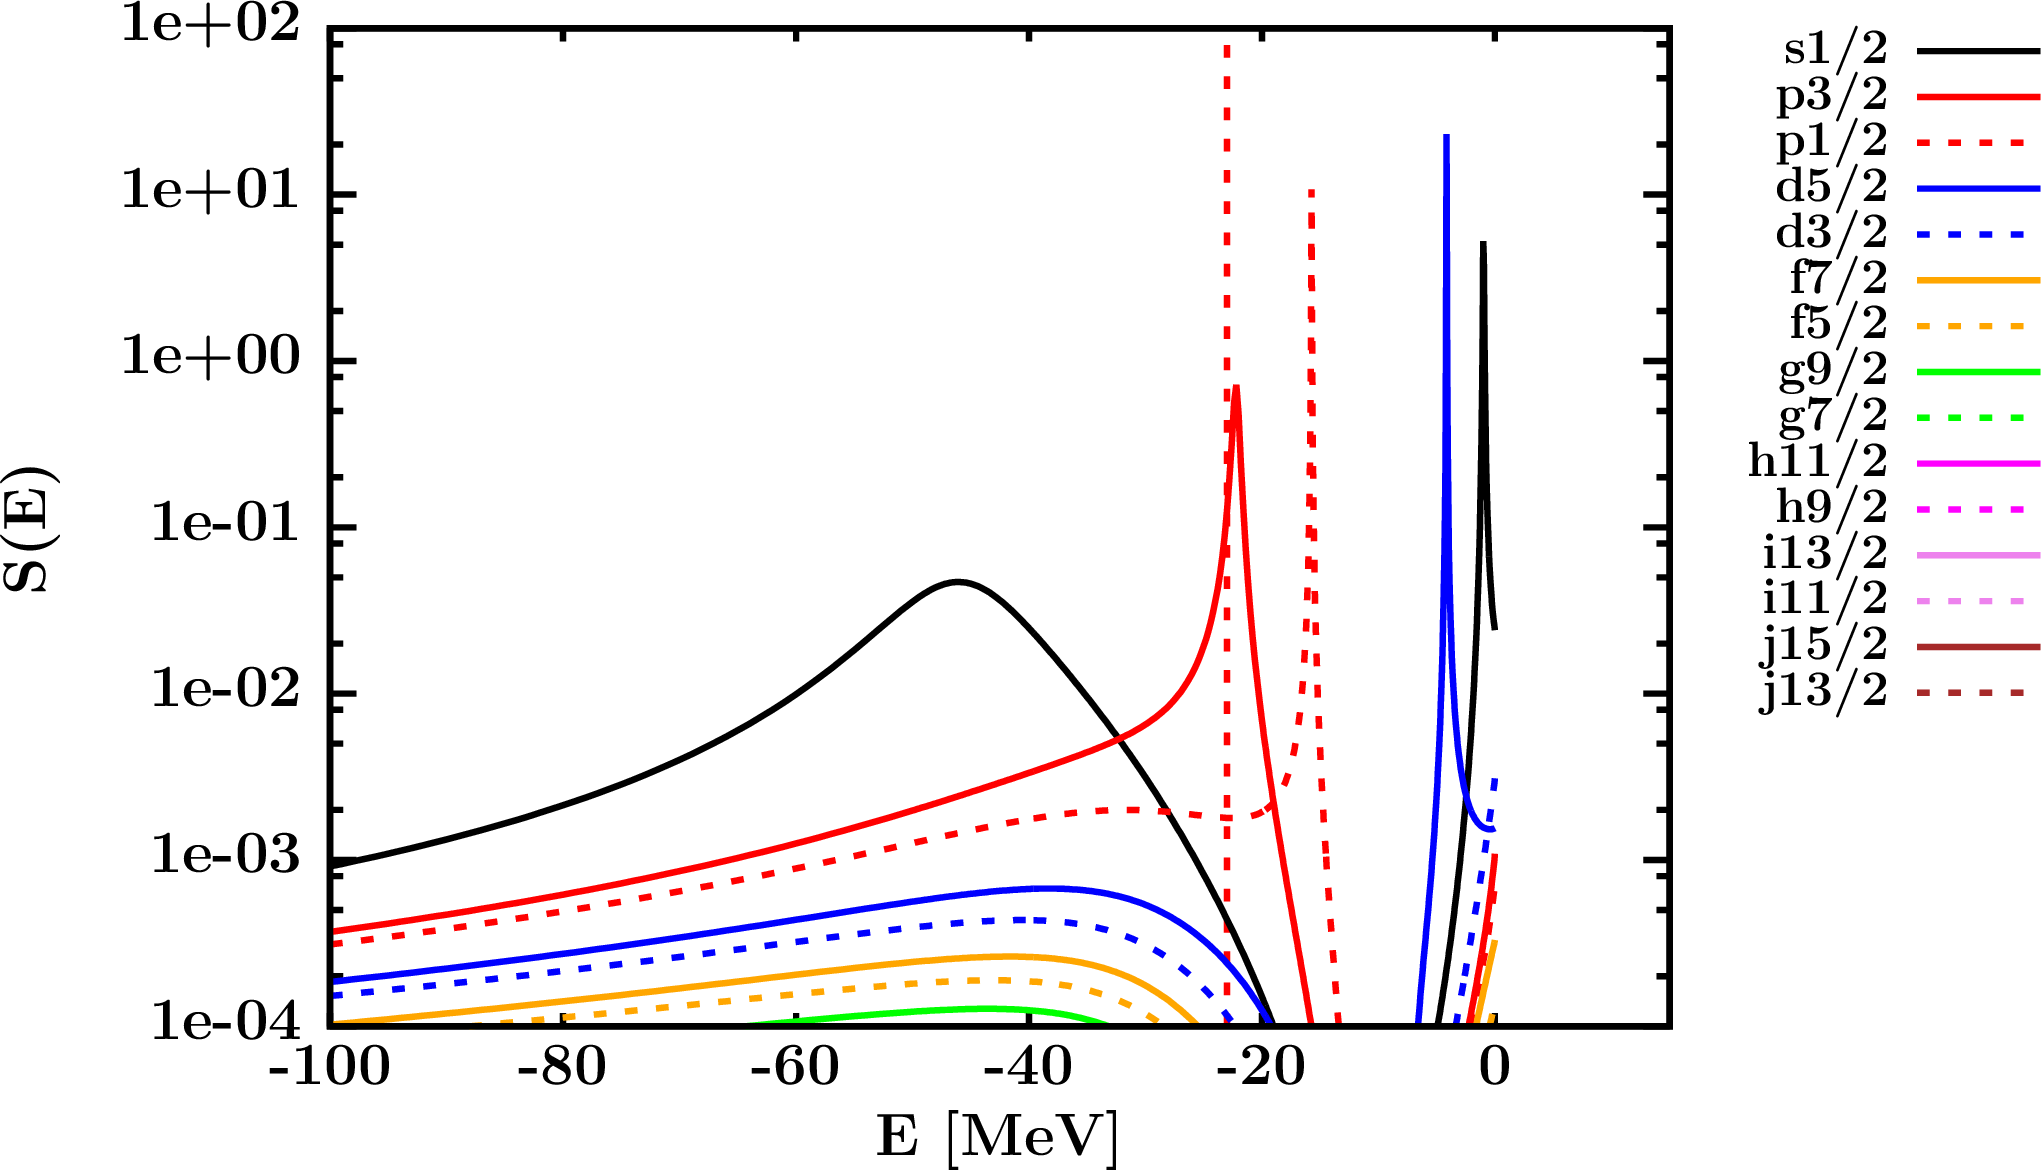
\includegraphics[width=1.0\textwidth]{figures/o16_neutronSpectralFunctions.png}
        \caption{Neutron spectral functions}
        \label{DOMFitData_o16_neutron_spectralFunctions}
    \end{minipage}
\end{figure}

\begin{figure}[H]
    \centering
    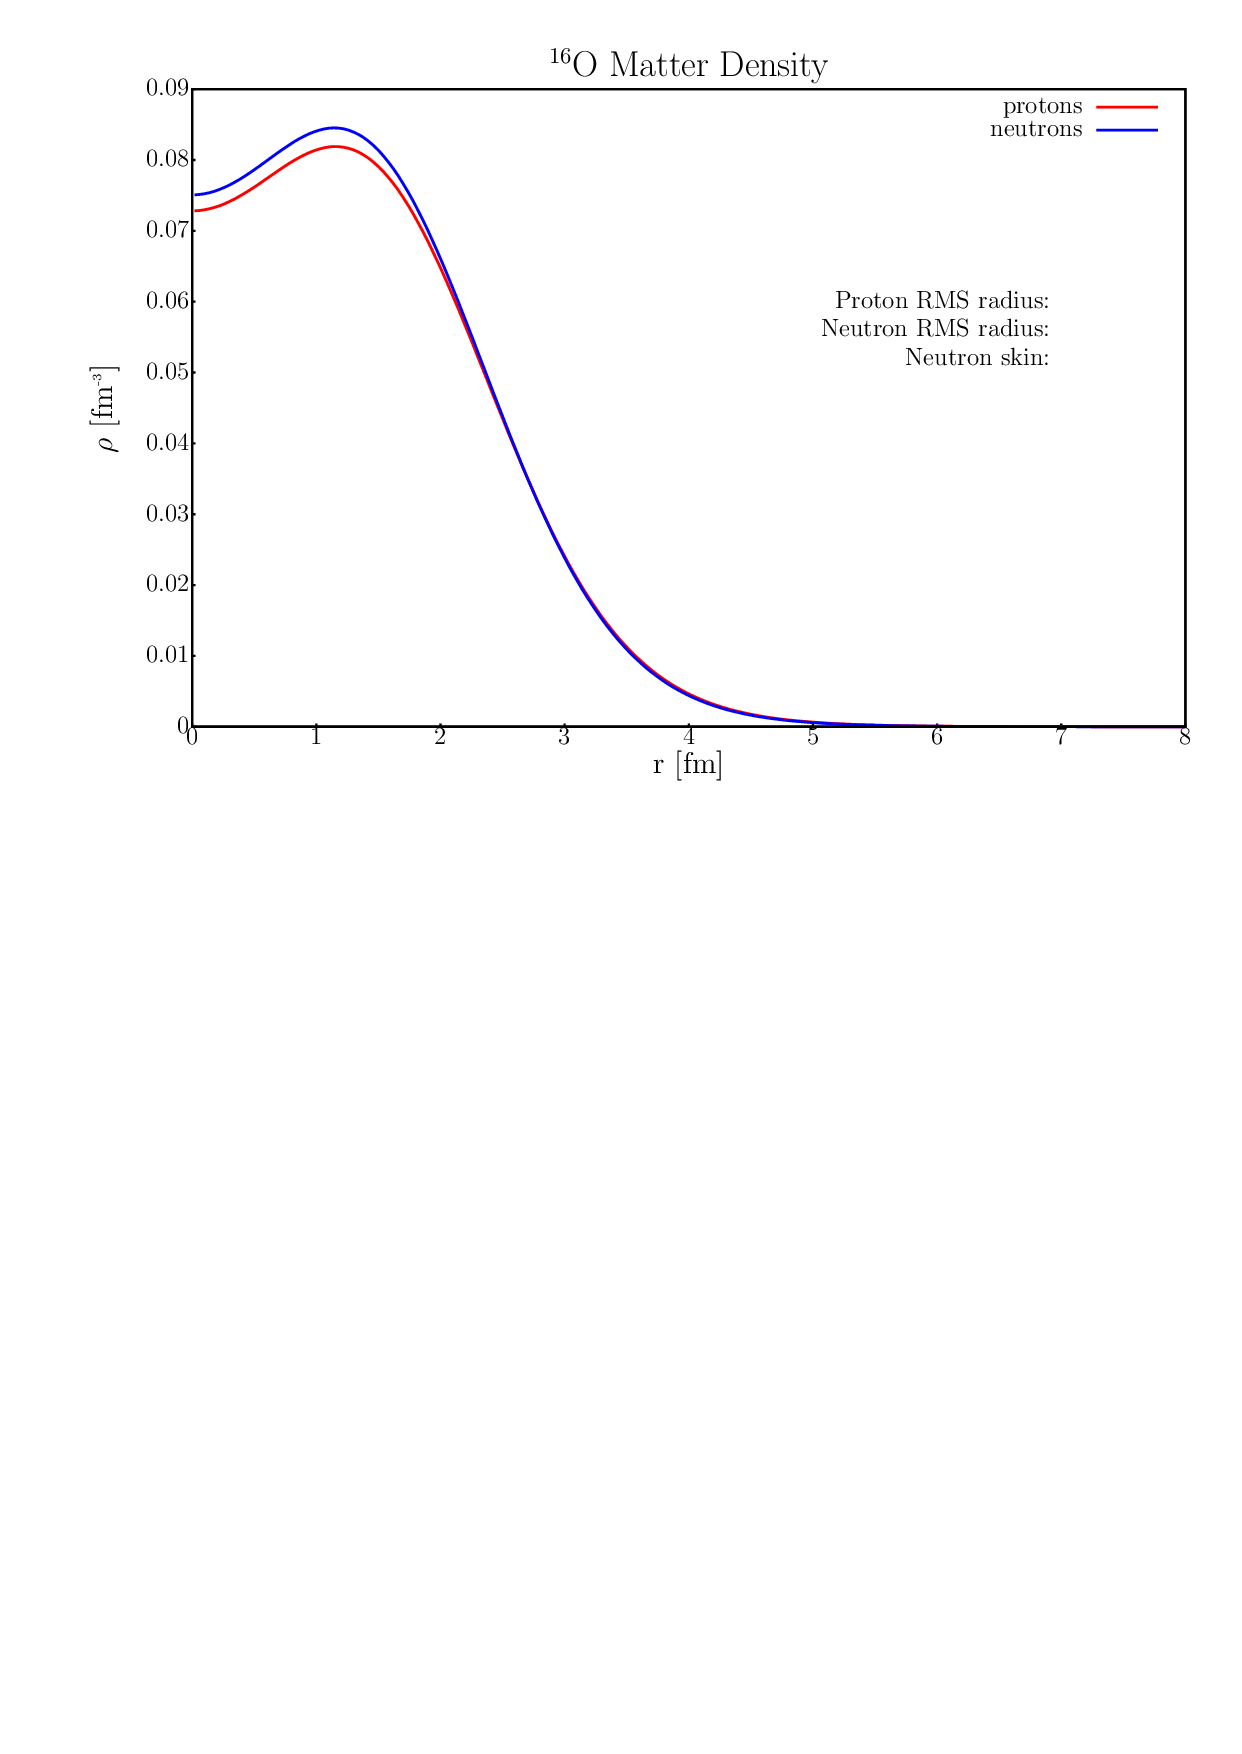
\includegraphics[width = 0.5\textwidth]{figures/o16_matterDensity.png}
    \caption{Matter density distribution}
    \label{DOMFitData_o16_matterDensity}
\end{figure}

\begin{figure}[H]
    \centering
    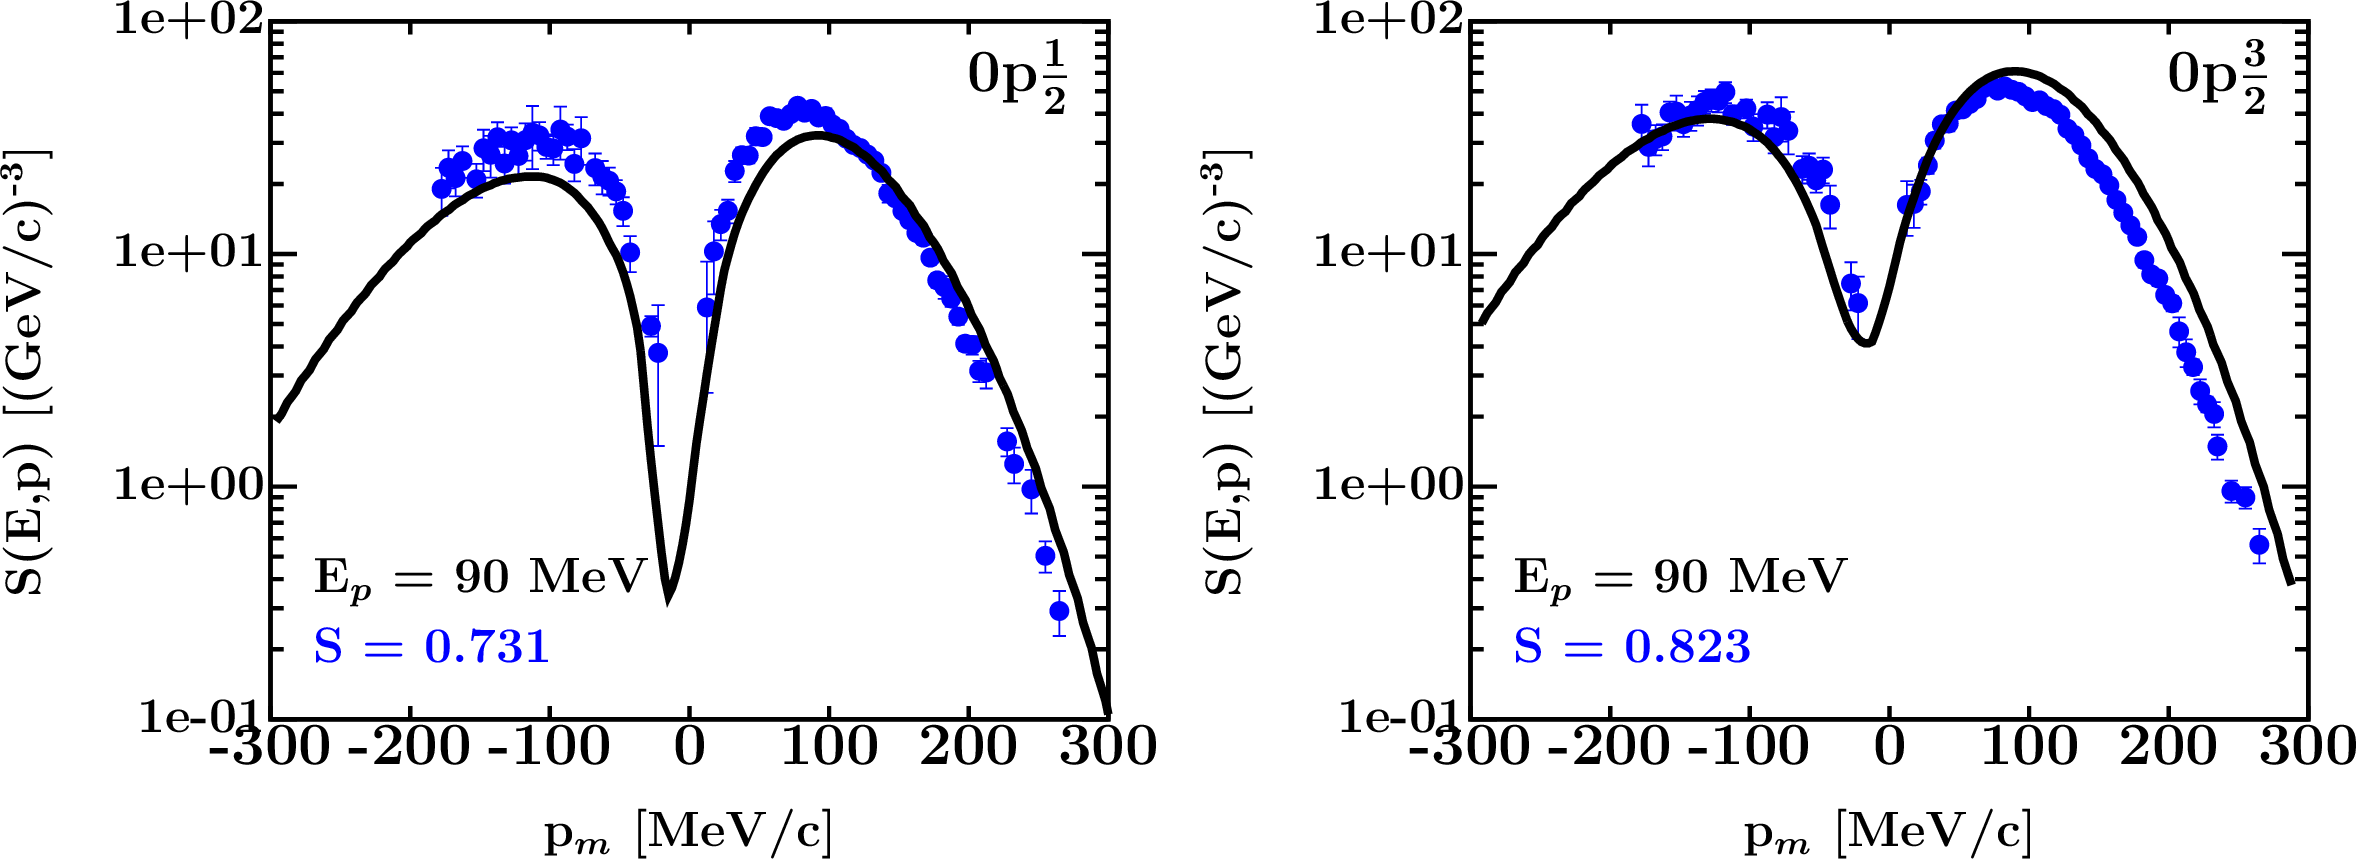
\includegraphics[width = 1.0\textwidth]{figures/o16_eep.png}
    \caption{(e,e'p) cross sections}
    \label{DOMFitData_o16_eep}
\end{figure}
